In what follows, several cases of application are presented to illustrate the versatility of BiorbdOptim and to give a practical overview on how to use the various features of the software.
The performances as well as the links to the detailed implementations of each example are listed in Tab.~\ref{tab:Perfs_and_detailed_implementations_of_each_example}.


\subsection{Muscle activation driven pointing task}

The goal of this example was to achieve a muscle activation driven pointing task with a 2-DoFs and 6-muscles arm model. 
The terms of the objective function are detailed in Tab.~\ref{tab:Muscle_activation_driven_pointing_task}.
The pointing tasks in itself resulted from the Mayer term ($\#1$, heaviest weight), which consisted in aligning two markers, the first one fixed in the ulna frame of reference and the second one fixed in the scene.
Terms $\#2$ and $\#3$ were added for control regularization while $\#4$ served as state regularization. 
In addition to muscle-induced torques, the formulation allowed additional pure torques directly at the joints to compensate for the weaknesses of the model.
The motion lasted for 2 seconds and was discretized using 51 shooting nodes.
%

%
\begin{table}[h!]
\caption{\small Muscle activation driven pointing task objective terms}
\label{tab:Muscle_activation_driven_pointing_task}
\centering
\begin{tabular}{c c c c}
\toprule 
& Type & Function & Weight \\ 
\midrule
$\#1$ & Mayer & ALIGN\_ MARKERS & $1e6$ \\ 
\midrule
$\#2$ & Lagrange & MINIMIZE\_ MUSCLE\_ CONTROL & $1e1$ \\ 
\midrule
$\#3$ & Lagrange & MINIMIZE\_ TORQUE & $1e1$ \\ 
\midrule
$\#4$ & Lagrange & MINIMIZE\_ STATE & $1e1$ \\
\bottomrule
\end{tabular}
\end{table}
%

%
The problem was solved with both solvers available (IPOPT and ACADOS) resulting in two significantly different solutions. 
Both are displayed in Fig.~\ref{fig:snapshots_activation_driven_pointing} to illustrate the pitfalls of local minima as well as the benefits of having access to several solvers with minimal effort.  
Indeed, the ACADOS solution (Fig.~\ref{fig:snapshots_activation_driven_pointing}, top) makes good use of gravity to minimize the control inputs, while the IPOPT solution (Fig.~\ref{fig:snapshots_activation_driven_pointing}, bottom) ends up with a much larger objective function, being struck in a local minimum (still achieving the task though). 
 
 
%
\begin{table}[h!]
\caption{\small Performance of each example and links to detailed implementations}
\label{tab:Perfs_and_detailed_implementations_of_each_example}
\centering
\begin{tabular}{c c c c}
&  & \multicolumn{2}{c}{Convergence time (s)} \\
\cmidrule[\heavyrulewidth]{3-4}
Example & Link & IPOPT & ACADOS \\ 
\midrule
Muscle activation driven pointing task & \href{https://github.com/pyomeca/BiorbdOptim/blob/master/examples/muscle_driven_ocp/static_arm.py}{$\star$} & $10.10$ & $0.2018$  \\ 
\midrule
$\bullet$ & $\bullet$ & $\bullet$ & $\bullet$ \\ 
\bottomrule
\end{tabular}
\end{table}
%

%
\begin{figure*}[t!]
\centering
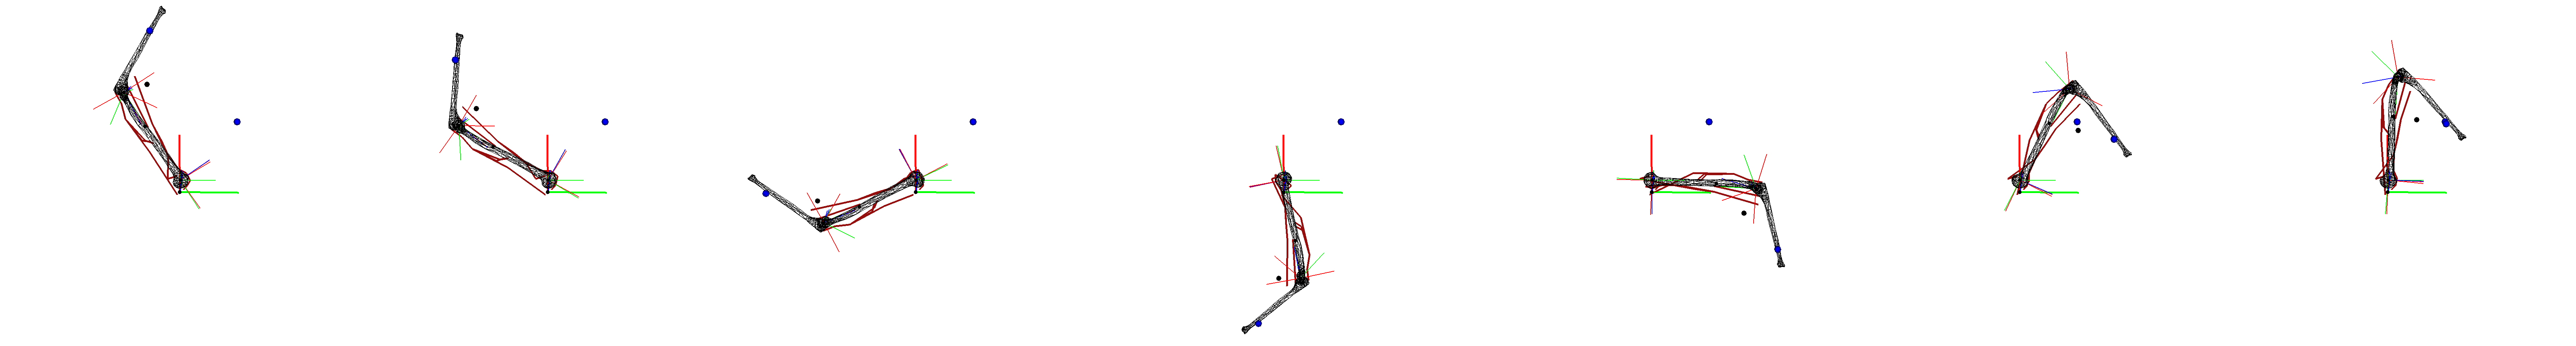
\includegraphics[width=\textwidth]{figures/activation_pointing_snapshots_acados.png}\\
\vspace*{0.5em}
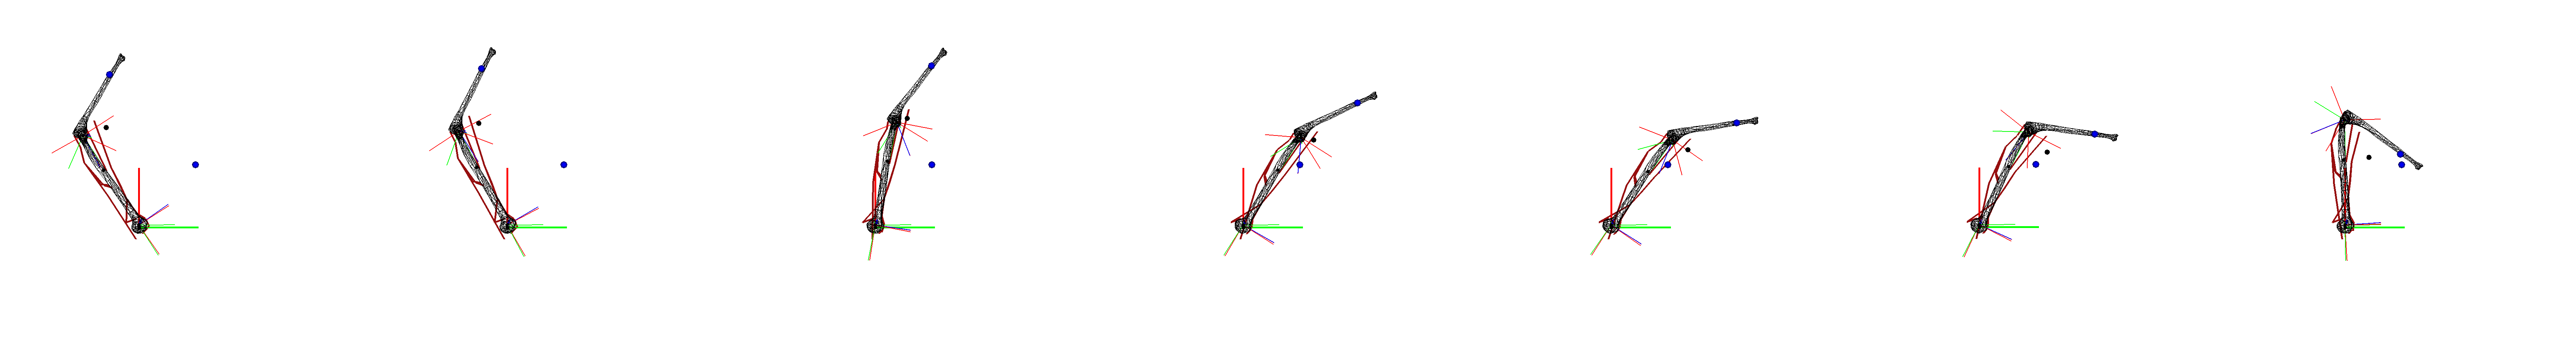
\includegraphics[width=\textwidth]{figures/activation_pointing_snapshots_ipopt.png}
\caption{Snapshots of an optimized muscle activation driven pointing task. Top: using ACADOS, optimized value = $427.5$. Bottom: using IPOPT, optimized value = $6959.3$.}
\label{fig:snapshots_activation_driven_pointing}
\end{figure*}
%